\documentclass[en]{../../../eplsummary}

\hypertitle{embedded-INGI2146}{8}{INGI}{2146}
{Gorby Nicolas Kabasele Ndonda\and Author2\and Author3}
{Professor}

\section{Introduction}
\begin{description}
    \item[Mobile:] Portable devices with wireless communication,
        running stand-alone or client applications.
    \item[Embedded:] An embedded system is a computer system with
        a dedicated function within a larger mechanical or electrical system.
\end{description}

Embedded systems are everywhere in smartphones, cars,\ldots Typical
characteristics is the following:
\begin{itemize}
    \item Cheap
    \item Reduced power consumption
    \item Real-time
    \item Robust
\end{itemize}

To achieve these characteristic, there need to be a tight coupling between
the hardware, the OS and the application.

\subsection{Real-Time Systems}

Real-Time Systems monitor and have an impact on the physical world via sensors
and actuators. Because of their nature, they have
requirements/constraints on timing:

\begin{description}
    \item[Hard constraint]
        \begin{itemize}
            \item Potentially severe consequences if reaction/result is produced after
                deadline.
            \item Results has no value (or even negative value) after deadline
        \end{itemize}
    \item[Firm constraint]
        \begin{itemize}
            \item Occasional miss tolerated, but degrades QoS
            \item No or little value after deadline
        \end{itemize}
    \item[Soft constraint]
        \begin{itemize}
            \item Result still has value after deadline
        \end{itemize}
\end{description}

\begin{center}
    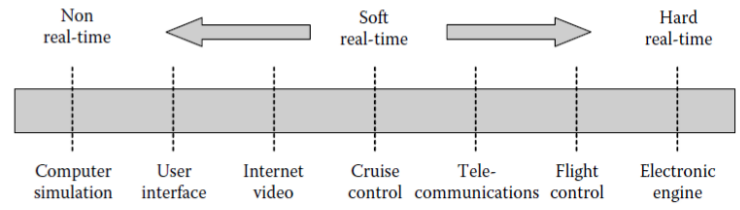
\includegraphics[width=0.7\linewidth]{img/realtime.png}
\end{center}

\subsection{Real-Time Tasks}
\begin{description}
    \item[Periodic:] Must be executed with fixed interarrival time
    \item[Sporadic:] Have known minimum interarrival time
    \item[Aperiodic:] No known interarrival time
\end{description}

\section{Wireless Sensor Networks}

Wireless Sensor Networks are composed of node (\textit{mote}) used for
monitoring and they communicates with each other and/or a remote server.

\subsection{Resource Constraint}
\begin{itemize}
    \item \textbf{Power}
        \begin{itemize}
            \item Batteries and Energy Harvesting
            \item Turn off idle devices
            \item Requires efficient OS and applications
            \item Reduce communication
        \end{itemize}

        \textit{Duty cycle} is the percentage of one period in which a
        signal or system active $\rightarrow$ isolated node will have
        high duty cycle

    \item \textbf{Bandwidth}
    \item \textbf{Memory}: just a few kBytes
    \item \textbf{CPU}: a few MHz
    \item \textbf{Data Transmission}: not enough power to reach server
        directly $\Rightarrow$ Multihop wireless Network
        \begin{itemize}
            \item Dynamic routing
            \item Self-Organizing Networks
        \end{itemize}
    \item Security: Not enough resources for sophisticated intrusion detection,
        encryption.
    \item Hardware: optimized
    \item \textbf{Reliable Data Flow}: Use 2-bit error correction and
        3-bit error detection.
        \begin{itemize}
            \item Store packet at source in circular buffer on flash 
            \item Remove data from source flash when End2End ack. (There
                is also data link ack)
        \end{itemize}
\end{itemize}

IoT = network of physical objects equipped with electronics and network
connectivity that can be sensed and controlled remotely.

\section{Operating Systems}

\subsection{Hardware}

\begin{description}
    \item[Microcontroller Unit]: Contains 
        \begin{itemize}
            \item CPU
            \item Memory (RAM and non-volatile)
            \item Interfaces to sensors and actuators
            \item Communication interfaces and interfaces to external memory
        \end{itemize}

    \item[JTAG] (Joint test action group): Allows to write code and data
        into flash memory or RAM of the MCU without using one of the
        communication interface
    \item[BSL] (Bootstrap Loader): similar JTAG but from a serial interface

        \begin{itemize}
            \item Can be used to debbuging code on the MCU from a PC
            \item Can upload code/data to the memory without any OS or program
                running.
        \end{itemize}

    \item[$\Rightarrow$] JTAG/BSL are useful for completely empty
        device where we can upload code/data without any OS.

    \item[Transceiver] Used to send data and receive data 
    \item[Interfaces and Sensors] Interfaces to sensor/Actuators
\end{description}

\subsection{Interrupts}
In order to make a software that react to the physical world two strategy:

\begin{description}
    \item[Polling] Read status of I/O every few milliseconds $\to$ waste of
        energy because CPU always busy

    \item[Interrupts] Signal to processor that current code execution should be interrupted
        because something important has happened.
        \begin{itemize}
            \item CPU stops execution and jumps to a specific place in the code that is 
                responsible for handling the interrupt
            \item Exist in all CPUs
            \item Handle by OS and device drivers
            \item Interrupts are expensive because of \textbf{context switching}
        \end{itemize} 
\end{description}

\subsection{OS for embedded systems}
OS are not necessary needed but they free the programmer from some concerns
\begin{itemize}
    \item Handle interrupts (events triggered when something happens)
    \item Manage memory
    \item Write your own process scheduler if you need multi-processing for
        background task
\end{itemize}

\paragraph{Linux}
Linux can be used for embedded systems but
\begin{itemize}
    \item requires enough memory 
    \item preemptive scheduling leads to latency for user code as
        kernel code cannot be preempted
\end{itemize}

\subsection{Real-Time OS}
OS specifically designed for real-time systems:
\begin{itemize}
    \item Much smaller than desktop/server OS
    \item Reduced set of functionality
    \item Fast context switch
    \item Guaranteed time-bounded response to interrupts
    \item Tries to avoid code that cannot be preempted
\end{itemize}

\subsection{OSs for WSN}
\begin{itemize}
    \item Thin abstraction layer to hardware(I/O, timers, \ldots)
    \item Limited multiprocessing
    \item Specific network protocol implementations
    \item Power saving
\end{itemize}

\subsubsection{TinyOS}
TinyOS applications consist of components that you can use in your own
application (as a \textit{set of libraries}). Each component is provided
with an interfaces defining the commands (function) and event available
in the component.

\begin{itemize}
    \item The device sleeps most of the time and they wake up when
        an event is triggered.
    \item Event-handling function execute and then device goes back to sleep.
\end{itemize}

\paragraph{Task}
Tasks are functions that can be preempted by interrupts but not by other tasks.
\begin{itemize}
    \item Task scheduler is a FIFO queue
    \item Not possible to post the same task while it is in the queue
    \item Device sleeps when task queue is empty and no event to process
\end{itemize}

\paragraph{Synchronous vs Asynchronous}
Hardware events can happen at any time and interrupt the current execution.
This can result in race conditions for variables shared between hardware and
task.
Compile differentiates between
\begin{itemize}
    \item Synchronous code: reachable only from tasks
    \item Asynchronous code: reachable from interrupts
\end{itemize}

Static analysis allows compiler to detect race conditions so programmer
are forced to explicitly use atomic section.

\paragraph{Optimization}
\begin{itemize}
    \item TinyOS programmed in NesC (subset of C)$\to$ No pointers or 
        dynamic allocation.
    \item Static analysis is used for optimization $\to$ can reduce apps by 60\%
\end{itemize}

\subsubsection{Contiki}
Differences with TinyOS
\begin{itemize}
    \item No special description language
    \item Cooperative process instead of task queue
    \item Core (kernal + libraries) is uploaded once
    \item Applications can be loaded at run-time
\end{itemize}
Application are composed of one or multiple processes. Proccesses are
cooperative, meaning that other processes can only run if current process
stops.
\begin{itemize}
    \item Processes communicate with each other by posting event
        \begin{itemize}
            \item Synchronous events: delivered immediately
            \item Asynchronous events: delivered later
        \end{itemize}
    \item Processes implemented as Proto-Threads
        \begin{itemize}
            \item Like threads but cheaper
            \item No separate stack per process $\to$ Local variables lose
                their value after a context switch
        \end{itemize}
    \item Process can be preempted by interrupts triggerd by hardware events.
\end{itemize}
\subsubsection{RIOT}
RIOT application programmed in C or C++ and used Multi-threading 
(not event-driven). $\to$ Use priority based scheduling.

\subsection{Networking Stacks}
uIP : Ipv4 stack in 4-5 KBytes of code.
\begin{itemize}
    \item One single packet buffer $\to$ easier to manage
    \item Incoming packet must be processed immediately $\to$ Radio interface queue
        incoming packet while processing.
    \item Retransmission is left to the application to recreate lost
        packet segments (not too bad if we considerer that packet
        contained sensor data, in this case new data are sent)
    \item Send segment one at the time, wait ACK before sending next segment

        $\Rightarrow$ saves memory, simplifies implementation but
        affects performance
    \item One single buffer for IP fragment reassembly
\end{itemize}


\section{TinyDB}
%%TODO


\section{Real-Time Scheduling}
\begin{description}
    \item[Job/processes/threads]: A task to be executed which compete for
        limited resource, the CPU
    \item[Scheduling:] Given N jobs, in which order should the CPU execute
        them
\end{description}

\paragraph{Scheduling goals}:

\begin{tabular}{lm{0.45\linewidth}m{0.45\linewidth}}
    & In general purposes OS( Linux,Windows, \ldots) &
    Real-time OS \\
    &
    \begin{description}
        \item[Fairness] All jobs should be finally executed (no starvation)
        \item[Optimize response time] Should be as short as possible on average
        \item[Optimize throughput] serve as many jobs as possible on average
            (Time to wait for CPU + Execution Time)
    \end{description}
    &
    In real-time system it's a bit different, the 
    \begin{itemize}
        \item most important thing is that task meets their deadline
        \item Don't care about fairness and throughput
        \item Focus on worst-case performance instead of average performance
    \end{itemize}
\end{tabular}

\subsection{Scheduling in general purpose OS}
Based on the idea of Round Robin scheduling which is preemptive with time
slice:
\begin{enumerate}
    \item All jobs wait in a queue for the CPU
    \item Job at the head of the queue receives service for time quantum Q
    \item Then it is interrupted by the next waiting job and goes back to the
        end of the queue
    \item Repeated until job is finished
    \item If Q is small, illusion of parallelism but careful of the cost for
        context switching
\end{enumerate}
By default all jobs are equal: order in queue is order of arrival and same time
slice for all jobs. But there are some variation with different priority and 
different time slice. Priority can be assigned manually or automatically

\subsection{Schedulability in real-time}
\begin{itemize}
    \item Given a set of tasks with their periods, deadlines, etc.
    \item Given a scheduling algorithm
    \item[$\Rightarrow$] The task set is \textbf{schedulable} if all jobs meet their deadlines.
\end{itemize}

Ways to know if task set is schedulable:
\begin{tabular}{l}
    Measurement on real system : expensive!\\
    Simulation\\
    \textcolor{red}{Mathematical analysis}\\
\end{tabular}

\paragraph{Assumption}
\begin{itemize}
    \item Single CPU
    \item No priority inversion
    \item Zero overhead for context switching
    \item Fixed number $N$ of independent periodic tasks with
        period $T_i$ and deadline $D_i$ (relative to begin of period), $i$=1,\ldots, $N$
    \item Task $i$ has a worst-case execution time $C_i$
\end{itemize}

\subsubsection{Rate Monotonic Scheduling}

RM is on \textcolor{red}{optimal} preemptive static priority scheduling
algorithm. It assigns a static priority to each task, the task with the shortest period
has highest priority. Preemption is possible.
\newline

Assuming $D_i=T_i$ for all tasks, a sufficient (but too pessimistic) test 
for schedulability with RM is:
$$\sum_{i=1}^N \frac{C_i}{T_i}\leq N(2^{\frac{1}{N}}-1)$$

\begin{center}
    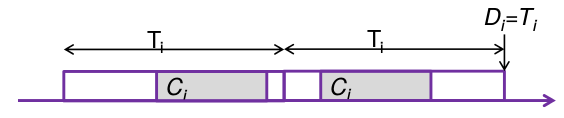
\includegraphics[width=0.5\linewidth]{img/RM.png}
\end{center}

RM is easy to implement with low overhead since task priorities are set at 
design time and does not change during run time but RM does not 
allow high CPU utilization because scheduling too rigid

\paragraph{Worst Case Execution Time}
To know worst case execution we can either do measurement or use static analysis

\subsubsection{Deadline Monotonic Scheduling}

RM does is not good for $D_i < T_i$, so in DM, task with shortest deadline
has highest priority. DM is on \textcolor{red}{optimal} preemptive static priority scheduling
algorithm for $D_i<T_i$.
$$\sum_{i=1}^N \frac{C_i}{D_i}\leq N(2^{\frac{1}{N}}-1)$$

        \begin{center}
            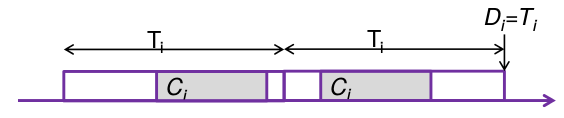
\includegraphics[width=0.5\linewidth]{img/RM.png}
        \end{center}

\subsubsection{Response Time Analysis}
RTA provides a sufficient and necessary test for all fixed-priority preemptive 
scheduling algorithms (RM,DM,\ldots)\\
A task set is schedulable if worst-case response time $R_i \leq D_i$ for all tasks.
\begin{itemize}
    \item Response time $R_i$ = $C_i + I_i$ where $I_i$ is the worst
        case interference time = amount of time a task is delayed by
        execution of higher priority tasks
\end{itemize}

\begin{eqnarray}
    R_i =& C_i + I_i\\
    R_i =& C_i + \sum_{j\in hp(i)} \lceil \frac{R_i}{T_j}\rceil C_j
    \label{rta-eq}
\end{eqnarray}

where hp(i) is the set of tasks with higher priotity than task i 
$\to \lceil \frac{R_i}{T_j}\rceil$ is the number of preemptions of task i by task j.



~\eqref{rta-eq} is a recursive formula so it is solve by finding smallest fixed point:
$$R_i^0 = C_i$$
$$R_i^{m+1} = C_i + \sum_{j \in hp(i)} \lceil \frac{R_i^m}{T_j}\rceil C_j$$

\subsubsection{Earliest Deadline First}

Optimal preemptive \textbf{dynamic} priority scheduling algorithm 
where task with earliest absolute deadline has the highest priority. The
absolute deadline is the time when the job is ready + $D_i$.

\subsection{Scheduling with resource lock}

We have assumed that task are independent, in a real systems, tasks can
be dependent because they access a shared resource in a critical section
(CS). In this case, a task with highest priority can be
\textbf{unboundedly} blocked by tasks with lower priority. Response time
becomes: $$R_i = C_i + I_i + B_i$$ where $B_i$ is the time the task is
blocked because a resource has been locked.

\begin{center}
    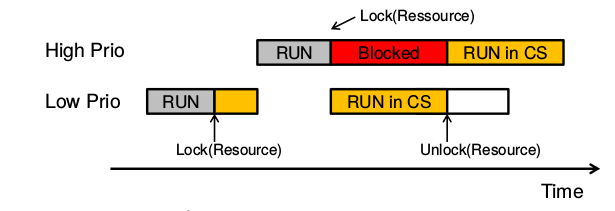
\includegraphics[width=0.5\linewidth]{img/priority.png}
\end{center}

\paragraph{Note:} RTA a test only sufficient, not necessary with blocking.

\paragraph{Priority inversion problem}

\begin{center}
    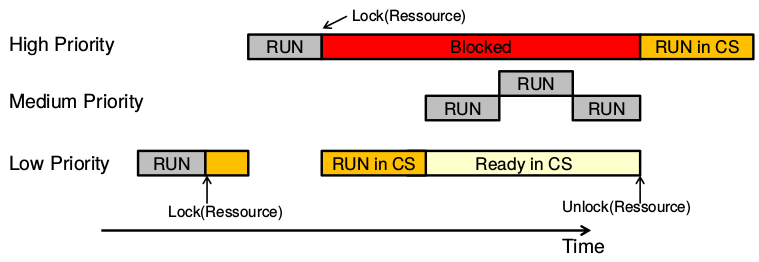
\includegraphics[width=0.5\linewidth]{img/inversion.png}
\end{center}

\subsubsection{Priority Inheritance Protocol}

To avoid this problem, a low-priority task inherits the priority of the 
blocked high-priority task.
\begin{itemize}
    \item When task i is blocked by a CS held by task k 
        and prio(i) > prio(k) $\to$ prio(k) := prio(i)
    \item When task k leaves the CS:
        \begin{itemize}
            \item If task k no longer blocks any tasks, it returns to its old priority
            \item If task k still blocks other tasks, it inherits their highest priority
        \end{itemize}
\end{itemize}

\subsubsection{Priority Ceiling Protocol}
Alternative to priority inheritance, a shared resource R can be accessed
only tasks $S_R = \{ t_1,\ldots,t_m\}$.
\begin{itemize}
    \item Assign a priority ceiling $C_R$ to that resource
        $$C_R = max_{t_i\in S}(prio(t_i))$$
    \item When a task locks that resource, its priority is immediately
        boosted to $C_R$
\end{itemize}

\paragraph{Note:}
Priority inheritance and priority ceiling require a scheduler that can handle
dynamic priorities

\subsection{Aperiodic/sporadic tasks}

\begin{itemize}
    \item \textbf{With hard deadlines}
        \begin{enumerate}
            \item \begin{itemize}
                    \item Take the lowest inter-arrival time L of those tasks
                    \item Treat them as a virtual periodic task with period L in 
                        schedulability analysis
                    \item[$\Rightarrow$]Too pessimistic
                \end{itemize}
        \end{enumerate} 

    \item \textbf{Without hard deadlines}
        \begin{enumerate}
            \item \begin{itemize}
                    \item Maintain the hard deadlines for the periodic tasks
                    \item Try to reduce response time for the other tasks
                \end{itemize}

                Simple and no impact on periodic tasks but possibly very
                long response times if the system is very busy with
                periodic task

            \item Polling server
                \begin{itemize}
                    \item A periodic task (''server'') with period $T_S$ to serve 
                        aperiodic/sporadic requests
                    \item Incoming aperiodic/sporadic jobs are queued in a queue
                    \item In one execution period, the server only runs up to $C_S$ time units
                \end{itemize}
                Performance can be controlled by the period and the priority of the server
                tasks and by $C_S$. 

                \begin{itemize}
                    \item Advantage: Polling server can be treated like a periodic task with
                        WCET $C_S$
                    \item Disadvantage: If an aperiodic/sporadic job is not handled by the
                        server in a time period, it has to wait for the next period $\to$ 
                        response time increases
                    \item Can be extended to multiple servers with different priorities,
                        periods and $C_S$ for different classes/types jobs.
                \end{itemize}
        \end{enumerate}
\end{itemize}
\end{document}
